

\section{Sistemos projektavimas}


\subsection{Reikalavimų surinkimas}
Programų sistemų architektūros yra reikalingos kuriant sistemas, kurios įgyvendina keliamus reikalavimus \cite{Bass2013}. Kadangi šio baigiamojo darbo tikslas - pasiūlyti architektūrą, todėl labai svarbu apsibrėžti keliamus sistemos reikalavimus. Šiame poskyryje bus pateikiami funkciniai ir nefunkciniai sistemos reikalavimai. Tam, kad apsibrėžti svarbius reikalavimus, reikia analizuoti dalykinę sritį, esamą situaciją. Surinkdamas reikalavimus, autorius remiasi 1 skyriuje identifikuotomis dalykinės srities problemomis, 2 skyriuje analizuotomis informacinėmis sistemomis ir nagrinėta literatūra.
\subsubsection{Funkciniai reikalavimai}

Funkciniai reikalavimai yra surinkti remiantis dalykinės srities analize ir identifikuotomis stacionaraus gydymo problemomis.

\begin{table}[!ht]
    \centering
    \renewcommand{\arraystretch}{1.2}
    \renewcommand\thetable{5}
    \caption{Projektuojamos sistemos funkciniai reikalavimai} 

    \begin{tabular}{|m{3em}|m{17em}|m{17em}|}
    \hline 
    \rowcolor[HTML]{EFEFEF} 
    Reik. Nr. & Reikalavimas & Aprašymas \\ \hline
    FR.1  &  Duomenų įvedimas galimas ALR technologijos pagalba  & Reikalavimas kyla iš stacionaraus gydymo problemų sprendimo būdų  (žiūrėti 2.3. poskyrį)    \\ \hline
    FR.2  &  Sistemos vidiniai naudotojai yra autorizuojami  &  Visi darbuotojai, kurie yra susiję su stacionariu gydymu,  yra identifikuojami, todėl svarbu, kad sistema autorizuotų naudotojus       \\ \hline
    FR.3  &  Sveikatos įstaigos darbuotojas, kuris turi atitinkamą rolę, gali sukurti gydymo planą  &   Reikalavimas kyla iš dalykinės srities (žiūrėti 1. skyrių)       \\ \hline
    FR.4  &  Pacientai yra identifikuojami ESPBI IS pagalba  &  Visų Lietuvos pacientų duomenys yra laikomi ESPBI IS, todėl sistema turi sugebėti komunikuoti su šia sistema      \\ \hline
    FR.5  &  Suteikta sveikatos paslauga yra identifikuojama  &   Reikalavimas kyla iš dalykinės srities (žiūrėti 1. skyrių)      \\ \hline
    FR.6  &  Kiekviena sąveika tarp slaugytojo ir paciento, kuri yra nurodyta gydymo plane, yra fiksuojama ir saugoma  &   Reikalavimas kyla iš dalykinės srities (žiūrėti 1. skyrių)       \\ \hline
    FR.7  &  Sveikatos įstaigos darbuotojas, kuris suteikė bet kokią sveikatos paslaugą, yra identifikuojamas  &   Reikalavimas kyla iš dalykinės srities (žiūrėti 1. skyrių)        \\ \hline
    
    \end{tabular}
\end{table}

\begin{table}[!ht]
    \centering
    \renewcommand{\arraystretch}{1.2}
    \renewcommand\thetable{5}

    \begin{tabular}{|m{3em}|m{17em}|m{17em}|}
    \hline 
    \rowcolor[HTML]{EFEFEF} 
    Reik. Nr. & Reikalavimas & Aprašymas \\ \hline
    FR.8  &  Medikamentų, kurie yra suteikiami pacientui, tinkamumo verifikavimas   &  Patikrinama ar suteikiamas medikamentas yra nurodytas gydymo plane ir neįvyko klaida. Reikalavimas kyla iš stacionaraus gydymo problemų sprendimo būdų  (žiūrėti 2.3. poskyrį)       \\ \hline
    FR.9  &  Paciento būklės duomenys, gauti suteikiant sveikatos paslaugą, yra fiksuojami ir saugomi  &    Reikalavimas kyla iš dalykinės srities (žiūrėti 1. skyrių)       \\ \hline
    FR.10  &  Formos, reikalingos stacionariame gydyme, yra pildomos sistemoje automatiškai, užpildant formą duomenimis, kurie buvo fiksuoti gydymo metu  &   Reikalavimas kyla iš stacionaraus gydymo problemų sprendimo būdų  (žiūrėti 2.3. poskyrį)       \\ \hline
    FR.11  &  Medicininių įrašų valdymo veiksmus gali atlikti tik tie darbuotojai, kurie turi valdymo veiksmams reikalingas roles  &  
    Slaugytojai gali redaguoti tik su jais susijusius įvestus duomenis, tačiau gydytojai gali redaguoti visus įvestus duomenis. Reikalavimas kyla iš dalykinės srities (žiūrėti 1. skyrių)       \\ \hline
    FR.12  &  Duomenų mainuose su centralizuota duomenų baze yra naudojamas HL7 formatas  &   Reikalavimas kyla iš sveikatos įstaigų informacinių sistemų analizavimo (žiūrėti 2.2.3 poskyrį)       \\ \hline
    \end{tabular}

\end{table}


\subsubsection{Nefunkciniai reikalavimai}
Nefunkciniai reikalavimai yra surinkti remiantis dabartinių sveikatos įstaigų naudojamomis informacinėmis sistemomis ir literatūra, kuri nagrinėja ALR panaudojimą sveikatos priežiūroje. Surinkti nefunkciniai reikalavimai apima šiuos reikalavimus:
\begin{itemize}
    \item Saugumo ir slaptumo reikalavimai;
    \item Ergonominiai reikalavimai;
    \item Prieinamumo ir patikimumo reikalavimai;
    \item Plečiamumo reikalavimai.
\end{itemize}

\begin{table}[!ht]
    \centering
    \renewcommand{\arraystretch}{1.2}
    \renewcommand\thetable{6}
    \caption{Projektuojamos sistemos nefunkciniai reikalavimai} 

    \begin{tabular}{|m{3em}|m{17em}|m{17em}|}
    \hline 
    \rowcolor[HTML]{EFEFEF} 
    Reik. Nr. & Reikalavimas & Aprašymas \\ \hline

    NFR.1  &  Vartotojo sąsaja turi būti pritaikyta neįgaliesiems pagal „Web Content Accessibility Guidelines 1.0“ pasiūlymus  &  Reikalavimas kyla remiantis ESPBI IS nagrinėjimu (žiūrėti 2.2. poskyrį)       \\ \hline
    NFR.2  &  Vartotojo sąsaja turi būti daugiakalbė &  Reikalavimas remiasi nagrinėtomis Lietuvos sveikatos įstaigų informacinėmis sistemomis (žiūrėti 2.1. poskyrį)       \\ \hline


    \end{tabular}

\end{table}

\begin{table}[!ht]
    \centering
    \renewcommand{\arraystretch}{1.2}
    \renewcommand\thetable{6}

    \begin{tabular}{|m{3em}|m{17em}|m{17em}|}
    \hline 
    \rowcolor[HTML]{EFEFEF} 
    Reik. Nr. & Reikalavimas & Aprašymas \\ \hline
    NFR.3  & Klaidų pranešimai formuojami taip, kad vartotojui būtų aišku kokių veiksmų imtis  &   Reikalavimas remiasi nagrinėtomis Lietuvos sveikatos įstaigų informacinėmis sistemomis (žiūrėti 2.1. poskyrį)       \\ \hline
    NFR.4  &  Sistemos integracija su skirtingomis sveikatos įstaigų informacinėmis sistemomis neturi būti sudėtinga  &   Reikalavimas remiasi nagrinėtomis Lietuvos sveikatos įstaigų informacinėmis sistemomis (žiūrėti 2.1. poskyrį)       \\ \hline
    NFR.5  &  Sistemos našumo plėtimas, gerinant ar didinant techninius išteklius, neturi būti sudėtingas, našumo plėtimas neturi reikalauti programos kodo keitimo  &   Reikalavimas kyla remiantis ESPBI IS nagrinėjimu (žiūrėti 2.2. poskyrį)       \\ \hline
    NFR.6  &   Sistema turi veikti pagal principą „24 valandos per dieną, 7 dienos per savaitę, 365 dienos per metus“  &  Reikalavimas kyla remiantis ESPBI IS nagrinėjimu (žiūrėti 2.2. poskyrį)       \\ \hline
    NFR.7  &  Sistemos, kuri susidūrė su sutrikimais, reikalaujančiais sistemos paleidimo iš naujo, prastovos laikas negali viršyti 3 valandų  &   Reikalavimas kyla remiantis ESPBI IS nagrinėjimu (žiūrėti 2.2. poskyrį)       \\ \hline
    NFR.8  &  Sistemos, kuri susidūrė su sutrikimais, reikalaujančiais sistemos diegimo iš naujo, prastovos laikas negali viršyti 6 valandų  &   Reikalavimas kyla remiantis ESPBI IS nagrinėjimu (žiūrėti 2.2. poskyrį)       \\ \hline
    NFR.9  &  Identifikavimo informacija turi būti šifruojama  &   Reikalavimas remiasi nagrinėtomis Lietuvos sveikatos įstaigų informacinėmis sistemomis (žiūrėti 2.1. poskyrį)       \\ \hline
    \end{tabular}

\end{table}

\subsection{Projektuojamos sistemos architektūra}
Programų sistemos architektūra, tai struktūrų rinkinys, kuris apima sistemos elementus, jų tarpusavio ryšius ir savybes \cite{Bass2013}. Kadangi visos programų sistemos turi architektūras \cite{Bass2013}, šiame poskyryje apžvelgiama projektuojamos sistemos architektūra.

\subsubsection{Projektuojamos sistemos priklausomybė nuo dabartinių sistemų}
Lietuvos sveikatos priežiūros įstaigas galima suskirstyti į dvi grupes - tiesiogiai naudojančios ESPBI IS ir netiesiogiai naudojančios ESPBI IS. Tiesiogiai ESPBI IS naudojančios įstaigos savo informacinės sistemos neturi, o netiesiogiai naudojančios įstaigos naudoja savo vidinę informacinę sistemą. Visos vidinės sistemos turi pacientų identifikavimo, duomenų saugojimo ir valdymo modulius. Šiame poskyryje nagrinėjama projektuojamos sistemos integracija su dabartinėmis sveikatos įstaigų vidinėmis informacinėmis sistemomis.

\textbf{Sistema yra posistemė dabartinių sistemų}. 2 skyriuje nagrinėtos sveikatos įstaigų informacinės sistemos yra sudarytos iš posistemių. Posistemes sudaro funkcionalumo aibės, kurios atitinka dalykinės srities poreikius, t.y. radiologijos reikmėms yra skirta radiologijos posistemė, laboratorijos reikmėms - laboratorijos posistemė, administravimo reikmėms - administravimo posistemė ir t.t. Kuriant sistemą, kaip dabartinės sistemos posistemę, reikėtų papildyti esamą vartotojo sąsaja su naujos posistemės teikiamais funkcionalumais, atlikti pakeitimus administravimo posistemėje. Taip pat gali būti neišvengiami kitų posistemių koregavimai. Jeigu projektuojama sistema būtų integruojama į daugiau sveikatos įstaigų, naująją sistemą reikėtų pritaikyti skirtingose informacinėse sistemos, nes skirtingos įstaigos turi skirtingas sistemas. Šis sistemos pasirinkimas reikštų, kad projektuojamą sistemą galėtų naudoti tik savo informacines sistemas turinčios sveikatos įstaigos. Tačiau kuriant tokią sistemą, didelė dalis reikalavimų, kilusių iš dalykinės srities, būtų įgyvendinti įstaigos informacinės sistemos, nereikėtų kurti modulių, kurių pagalba komunikuojama su ESPBI IS.

\textbf{Sistema nėra priklausoma nuo dabartinių sistemų}. Kadangi ne visos sveikatos įstaigos turi savo vidines informacines sistemas, viena iš alternatyvų - kurti sistemą, kuri visus keliamus reikalavimus įgyvendintų pati ir nebūtų priklausoma nuo dabartinių įstaigų vidinių sistemų. Kadangi visos sveikatos įstaigos yra dalinai priklausomos nuo ESPBI IS suteikiamų duomenų, todėl visos sistemos, manipuliuojančios šiais duomenimis, privalo komunikuoti su ESPBI IS. Vadinasi, kuriama sistema turėtų pati valdyti duomenų mainus. Projektuojamos sistemos funkcionalumo poaibis sutaptų su dabartinių sistemų funkcionalumų poaibiais. Tokią sistemą galima būtų diegti tiek į įstaigas, kurios neturi vidinių informacinių sistemų, tiek į tas, kurios turi. Diegiant sistemą į įstaigas, kurios turi vidines informacines sistemas, nereikėtų papildomų kaštų vidinių sistemų koregavimui ir jų pritaikymui projektuojamai sistemai, todėl diegimas į visas įstaigas būtų vienodas. Jeigu būtų pasirinkta ši sistema, atsirastų daug funkcionalumo ir duomenų dubliavimo, tačiau ši problema kiltų tik tose įstaigose, kurios turi vidines sistemas. Taip pat šios sistemos kūrimo kaštai būtų didesni nei pirmojo pasiūlymo, nes reikėtų implementuoti daugiau funkcionalumų ir atsirastų duomenų bazė, kurioje būtų laikomi sistemai reikalingi duomenys, kurie nėra gaunami iš ESPBI IS.

\textbf{Sistema yra dalinai priklausoma nuo dabartinių sistemų}. Vienas iš pasirinkimų galėtų būti dalinis sistemos priklausomumas nuo dabartinių sistemų. Projektuojama sistema pati nedalyvautų duomenų mainuose su ESPBI IS, tačiau turėtų tarpinį sluoksnį, kuris bendrautų su dabartinių sistemų duomenų mainų sluoksniu. Šis lygmuo pasirūpintų, kad sistema gautų norimus duomenis. Likusi sistemos dalis būtų savarankiška ir nepriklausytų nuo kitų sistemų, t.y. suprogramavus vartotojo sąsają bei įgyvendinus visus funkcionalumus, jų pritaikyti dabartinėms sistemoms nereikėtų. Diegiant sistemą į skirtingas sveikatos priežiūros įstaigas, kurios turi vidines sistemas, reikėtų koreguoti tik sistemų sąlyčio taškus, t.y. projektuojamos sistemos tarpinis sluoksnis ir vidinių sistemų duomenų mainų sluoksniai. Jeigu sveikatos įstaiga neturi vidinės sistemos, papildomai reikėtų suprojektuoti ir įdiegti duomenų ir duomenų mainų sistemą. Jeigu būtų pasirinkta ši sistema, būtų išvengiamas funkcionalumų ir duomenų dubliavimas. Tačiau kiekvienai vidinei sistemai reikėtų pritaikyti naująją sistemą, o jeigu nėra vidinės sistemos, reikėtų papildomų kaštų trūkstamoms sistemos dalims suprojektuoti ir sudiegti.

Norint projektuoti sistemą, kuri būtų posistemė dabartinių sistemų, reikėtų išsikelti prielaidą, kad sistema yra diegiama tik tuose sveikatos įstaigose, kuriose veikia vidinės informacinės sistemos. Pasirinkus šį pasiūlymą ne tik sumažėtų sveikatos įstaigų, kuriose galima pritaikyti sistemą, skaičius, bet ir kiekvienos įstaigos vidinei sistemai reikėtų pakeitimų. Norint išvengti minėtų problemų, galima kurti sistemą, kuri nėra priklausoma nuo dabartinių sistemų. Tačiau susidurtume su naujomis problemomis - funkcionalumo bei duomenų dubliavimo ir didesnių sistemos kūrimo kaštų. Paskutinis pasiūlymas, kur sistema yra dalinai priklausoma nuo dabartinių sistemų, spręstų visas minėtas problemas, išskyrus vidinių sistemų pakeitimus, todėl šis pasirinkimas yra tinkamiausias.
% \subsubsection{Prielaidos}
% \textbf{IT} infrastruktūra. Lieuvos sveikatos priežiūros įstaigas galima suskirstyti į dvi grupes - tiesiogiai naudojančios ESPBI IS ir netiesiogiai naudojančios ESPBI IS. Tiesiogiai ESPBI IS naudojančios įstaigos savo informacinės sistemos neturi, o netiesiogiai naudojančios įstaigos naudoja savo vidinę informacinę sistemą. Visos vidinės sistemas turi pacient identifikavimo, duomenų saugojimo ir valdymo modulius.

% zmones turi bazines kompiuterio naudojimo zinias

\subsubsection{Architektūros stilius}
Šiame poskyryje apžvelgiami galimi būsimos sistemos architektūros stiliai. Taip pat pasirenkamas tinkamiausias stilius iš apžvelgtųjų. 

\textbf{Komponentais pagrįstas architektūros stilius}. Komponentinis architektūros stilius yra pagrįstas sistemos išskaidymu į smulkesnius funkcinius ir loginius elementus, kurie yra vadinami komponentais. Jungiant komponentus tarpusavyje, gaunama pilna sistema. Kiekvienas komponentas turi apsibrėžęs komunikavimo sąsają (angl. \textit{interface}), kurioje nurodomi kokie komponento įgyvendinti metodai yra pasiekiami kitiems komponentams. Vienas iš pagrindinių šios architektūros bruožų - komponentų perpanaudojimas. Kadangi kiti komponentai komunikuoja tik per komponento sąsają, komponentą yra lengva pakeisti kitu komponentu, turinčiu tokią pačia sąsają. Kuriant sistemą, kurios architektūros stilius būtų komponentinis, susidurtume su dideliais sistemos kaštais \cite{Component}, nes perpanaudojamų komponentų kūrimas pareikalautų daug laiko ir pastangų, o tai reikštų kaštų didėjimą.

\textbf{Daugiasluoksnės architektūros stilius}. Šis architektūros stilius yra pagrįstas sistemos skaidymu į loginius sluoksnius ir fizinius lygmenis. Kiekvienas sluoksnis turi savo rolę ir atsakomybę (pvz.: verslo logikos, vaizdavimo ir t.t.), todėl kiekvienas sluoksnis atlieka veiksmus susijusius tik su jo logika, o kitų sluoksnių logika jam nėra aktuali. Fiziniai lygmenys yra atskirti fiziškai, t.y. kiekvienas fizinis lygmuo veikia ant skirtingų kompiuterių, tačiau vienam fiziniame lygmenyje gali būti keletas loginių sluoksnių. Tokia architektūra leidžia sistemai būti tiek vertikaliai, tiek horizontaliai plečiamai \cite{By}. Taip pat ši architektūra yra paprastesnė nei komponentinė, todėl jos kūrimo kaštai yra mažesni. Tačiau augant sluoksnių skaičiui, sistemos sudėtingumas ir kūrimo kaina didėja.

\textbf{Netaikyti architektūros stilių}. Taip pat vienas iš variantų, sistemos architektūros stiliaus pasirinkime, yra visai netaikyti architektūros stilių. Toks pasirinkimas leistų greitai sukurti sistemą, nes kūrimo metu nereikėtų laikytis taisyklių ir nevaržytų apribojimai, kurie kyla iš architektūrų stilių. Kadangi šis pasirinkimas leistų sistemą greitai sukurti, vadinasi jos kūrimo kaštai nebūtų dideli. Jeigu nebūtų taikomas joks architektūros stilius, vadinasi sistema būtų labai sunkiai plečiama, o auganti techninė skola (angl. \textit{techincal debt}) didintų sistemos palaikymo kaštus, todėl sistemos bendra kūrimo ir palaikymo kaina būtų didelė. Ši alternatyva nėra laikoma geros architektūros praktika \cite{Bass2013}.

Renkantis sistemos architektūros stilių, svarbu atkreipti dėmesį į sistemai keliamus reikalavimus, taip pat atkreipti dėmesį į sistemos kaštus. Jeigu pasirinktume netaikyti jokio stiliaus, vadinasi sistemą sukurti nebus brangu, tačiau jos palaikymo kaštai bus dideli. Jeigu pasirinktume komponentinį architektūros stilių, sistemos architektūra būtų sudėtinga, o sistemos kūrimo kaštai dideli. Daugiasluoksnės architektūros stilius leistų sistemai būti plečiamai bei sistemos kaštai būtų mažesni nei komponentinės, todėl šis stilius yra tinkamiausias kuriant siūlomą sistemą.


\subsubsection{ALR skaitytuvas ir sistemos vartotojo sąsaja}

Teigiama, jog nuo 2015 metų, 50\% rinkoje naudojamų mobiliųjų telefonų turi įdiegtą ALR technologiją \cite{forum2}. Taip pat dauguma literatūros šaltinių, kurie analizuoja sveikatos priežiūrą ir ALR technologiją, renkasi mobilųjį telefoną kaip ALR skaitytuvą \cite{Azlina2013} \cite{Strommer2006} \cite{Puma2012} \cite{Marcus} \cite{Gautam}. Malaizijoje atlikta apklausa rodo, kad didžioji dalis sveikatos priežiūros įstaigų darbuotojų rinktųsi naudoti mobiliuosius telefonus kaip ALR skaitytuvus \cite{Azlina2013}. Kadangi dauguma mobiliųjų telefonų turi įdiegtą ALR technologiją ir literatūros šaltiniuose siūloma juos panaudoti ALR įgalintose sistemose, mobilusis telefonas būtų tinkamas projektuojamos sistemos ALR skaitytuvas. Kadangi duomenis, kurie yra įvesti į sistemą, galima matyti ir koreguoti, sistemos naudojimui reikalinga vartotojo sąsaja. Toliau šiame poskyryje apžvelgiami vartotojo sąsajos dislokavimo variantai.

\textbf{Vartotojo sąsaja ALR skaitytuve}. Kliento sluoksnis ir ALR valdiklių sluoksnis gali būti viename lygmenyje, t.y. tiek vartotojo sąsaja, tiek ALR skaitytuvas gali būti viename įrenginyje. Nuskaičius ALR žymą, naudotojas iš karto gali matyti įvestus duomenis, juos redaguoti, išsaugoti. Naudotojui tai būtų patogu, nes jis visus sistemos funkcionalumus gali pasiekti viename įrenginyje. Pasirinkus šį sprendimą, jeigu ALR skaitytuvas būtų nedidelio dydžio, naudotojui gali kilti nepatogumų pildant, redaguojant ir skaitant formose pateiktus duomenis.

\textbf{Vartotojo sąsaja kompiuterio programinėje įrangoje ir ALR skaitytuve}. Taip pat vartotojo sąsaja gali būti kaip kompiuterio programinė įranga. Nuskaičius ALR žymą, nuskaityti duomenys atsirastų kompiuterio programinėje įrangoje, kur vartotojas galėtų duomenis redaguoti, peržiūrėti ir išsaugoti. Jeigu būtų pasirinktas šis variantas, kiekviename kompiuteryje reikėtų įdiegti šią programinę įrangą. Taip pat, programinę įrangą reikėtų kurti skirtingoms kompiuterių operacinėms sistemoms, o tai padidintų kuriamos sistemos kaštus. Kadangi ALR žymos būtų nuskaitomos su vienu įrenginiu, o duomenų redagavimas ir vaizdavimas atliekamas su kitu, naudotojui gali kilti nepatogumų vaikštant nuo paciento iki artimiausio kompiuterio. Tačiau tuo atveju, kuomet duomenų redagavimui interakcija su paciento ALR žyme nėra reikalinga, naudotojui būtų patogiau redaguoti duomenis naudojantis kompiuteriu, o ne mobiliuoju telefonu. 

\textbf{Vartotojo sąsaja interneto naršyklėje ir ALR skaitytuve}. Kadangi šiuo metu interneto naršyklė yra įdiegta tiek į stacionarius ir nešiojamus kompiuterius, tiek į mobiliuosius telefonus bei planšetinius kompiuterius, projektuojamos sistemos vartotojo sąsaja, kurioje naudotojai gali redaguoti duomenis, galėtų būti pasiekiama per interneto naršyklę. Šis sprendimas leistų išvengti skirtingų operacinių sistemų keliamų sunkumų. Jeigu vartotojo sąsaja būtų pritaikyta mažiems įrenginiams (angl. \textit{responsive}), sistema būtų patogu naudotis neatsižvelgiant į įrenginio dydį. Kadangi ALR skaitytuvas būtų įdiegtas mobiliajame telefone, pasirinkus šį variantą, naudotojas galėtų duomenų redagavimo operacijoms naudoti arba ALR skaitytuvą, arba kitą įrenginį. 


Visų nagrinėtų informacinių sistemų (žiūrėti 2. skyrių), kurios yra naudojamos sveikatos priežiūros įstaigų darbuotojų, vartotojo sąsajos yra pasiekiamos interneto naršyklėje. Todėl tikėtina, kad įstaigos darbuotojams būtų patogiau naudotis sistema, jeigu jie turėtų galimybę redaguoti duomenis interneto naršyklėje. Kadangi siūloma naudoti mobilųjį telefoną kaip ARL skaitytuvą, naudotojai galėtų pasirinkti ar duomenis koreguoti mobiliajame telefone, ar kompiuteryje. Dėl išvardintų priežasčių, vartotojo sąsaja interneto naršyklėje ir ALR skaitytuve yra tinkamiausias variantas.

\subsubsection{Medikamentų išdavimas}
Medikamentų išdavimo procedūra yra viena iš pagrindinių stacionaraus gydymo paslaugų (žiūrėti 1. skyrių). Šiame poskyryje pateikiama medikamentų išdavimo sekų diagrama (žiūrėti 4 pav.). Šios procedūros tikslas - išduoti medikamentą pacientui ir užfiksuoti šį faktą medicininiu įrašu. Šios diagramos pirminis agentas - sistemos naudotojas, t.y. slaugos darbuotojas arba gydytojas. Šią sekų diagramą sudaro 29 žingsniai.

\begin{figure}[H]
    \centering
    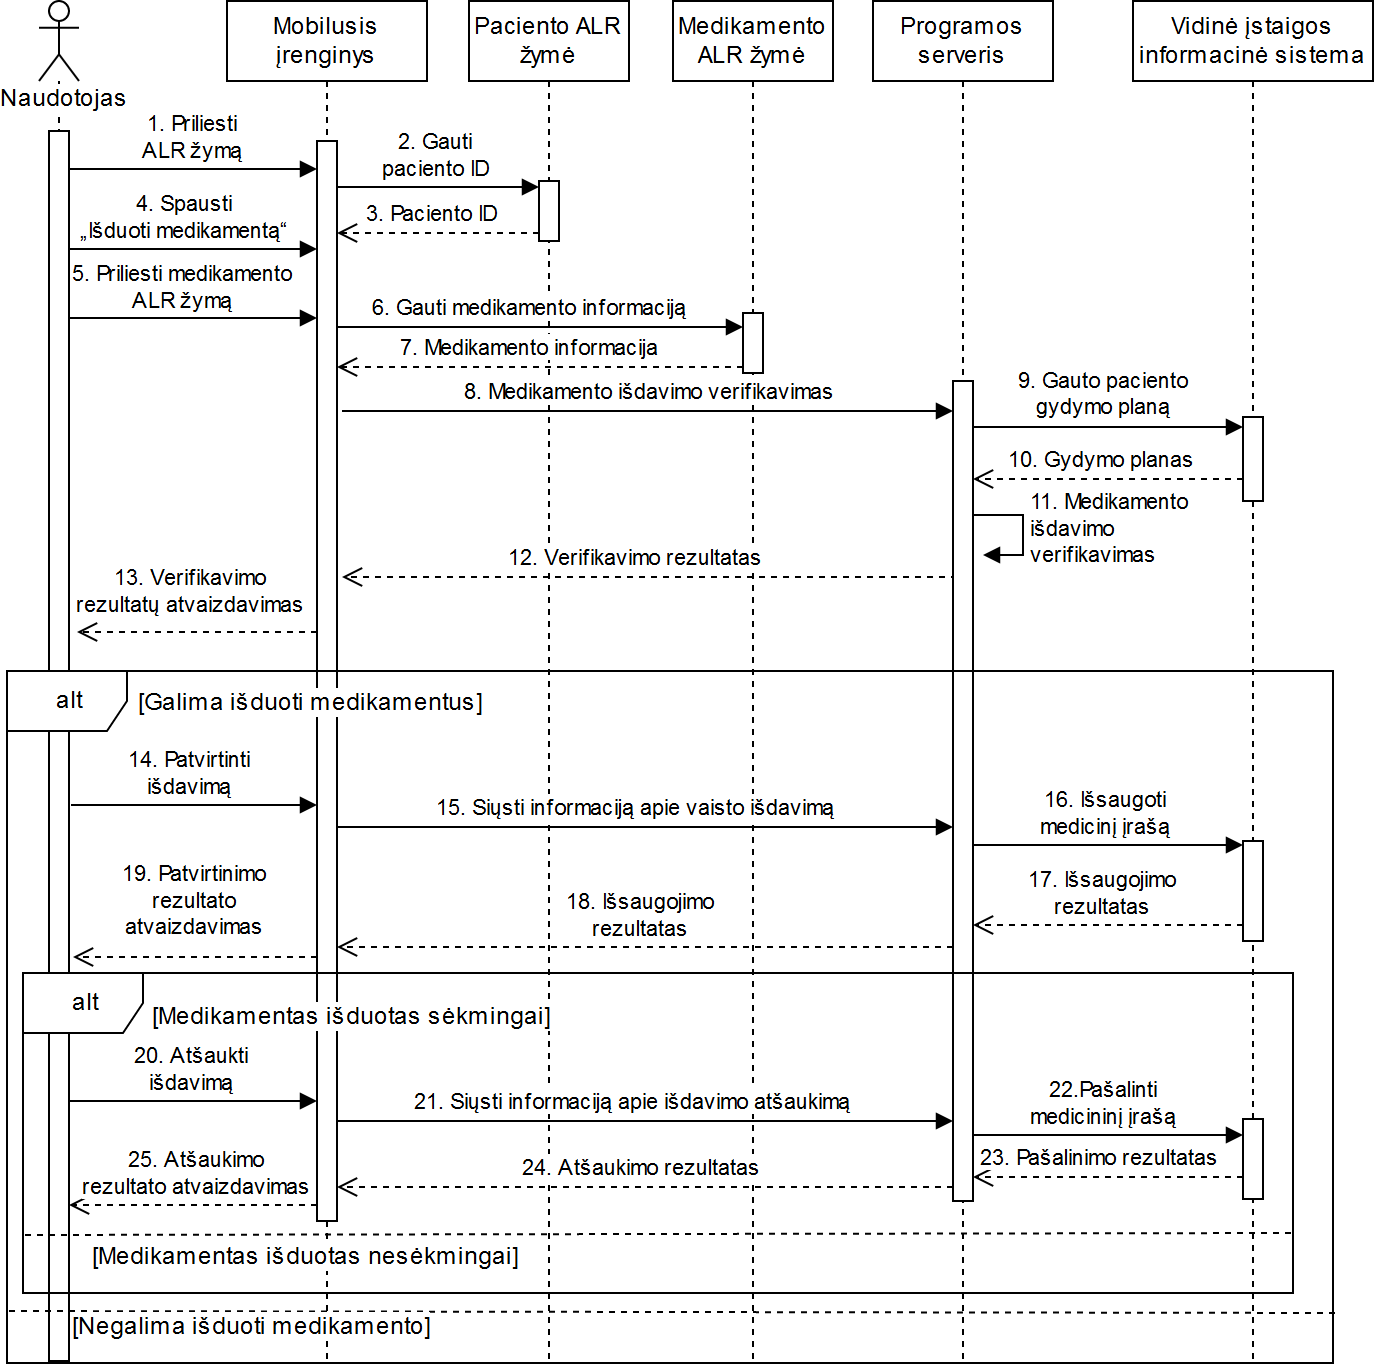
\includegraphics[scale=0.27]{images/israsytiVaistai}
    \caption{Medikamentų išdavimo sekų diagrama} 
\end{figure}

Medikamentų išdavimo procedūrą gali sudaryti mažesnis žingsnių kiekis, toliau pateikiamos šios procedūros žingsnių alternatyvos.


\textbf{Atsisakyti „Išduoti medikamentą“ ir „Patvirtinti“ mygtukų}. Atsisakius šių dviejų mygtukų paspaudimo, naudotojui vietoj 5 žingsnių, šiai procedūrai atlikti užtektų 3 žingsnių. Tačiau sumažėjus naudotojo žingsnių kiekiui, naudotojui gali tapti neaišku kokį sekantį žingsnį jis turi atlikti, nes nuskaičius paciento ALR žymą, intuityviai reikėtų žinoti, kad iš karto reikia priliesti ir medikamento ALR žymą. Jeigu šių mygtukų nebūtų, naudotojui gali kilti keblumų kuomet nuskaitoma keleto pacientų ALR žymos ir tuomet nuskaitoma medikamento ALR žyma. Šio scenarijaus atveju gali kilti neaiškumų dėl konkretaus paciento, kuriam turėjo būti išduotas medikamentas.

\textbf{Paciento gydymo plano informaciją laikyti ALR žymoje}. ALR žymoje laikant visą reikiamą informaciją apie paciento gydymo planą, sutrumpėtų uždelsimo laikas, kuris susidaro vykdant 9 ir 10 žingsnius. Pasirinkus šią alternatyvą, reikėtų atkreipti dėmesį į paciento duomenų saugumą. Kadangi paciento gydymo planas yra konfidencialus dokumentas, plano duomenų pasiekiamumas negali būti viešas. Reikėtų užtikrinti, kad tik sistemos ALR skaitytuvai galėtų gauti ir iššifruoti gydymo plano duomenis.

\subsubsection{Paciento būklės fiksavimas}
Kadangi viena iš stacionaraus gydymo pagrindinių procedūrų - paciento gyvybinių požymių fiksavimas, t.y. širdies ritmo, temperatūros ir kitų rodiklių fiksavimas, žemiau pateikiama šios procedūros sekų diagrama (žiūrėti 5 pav.). Šios procedūros tikslas - gydymo plane nurodytų paciento būklės požymių fiksavimas. Šios diagramos pirminis agentas - sistemos naudotojas, t.y. slaugos darbuotojas arba gydytojas.

\begin{figure}[H]
    \centering
    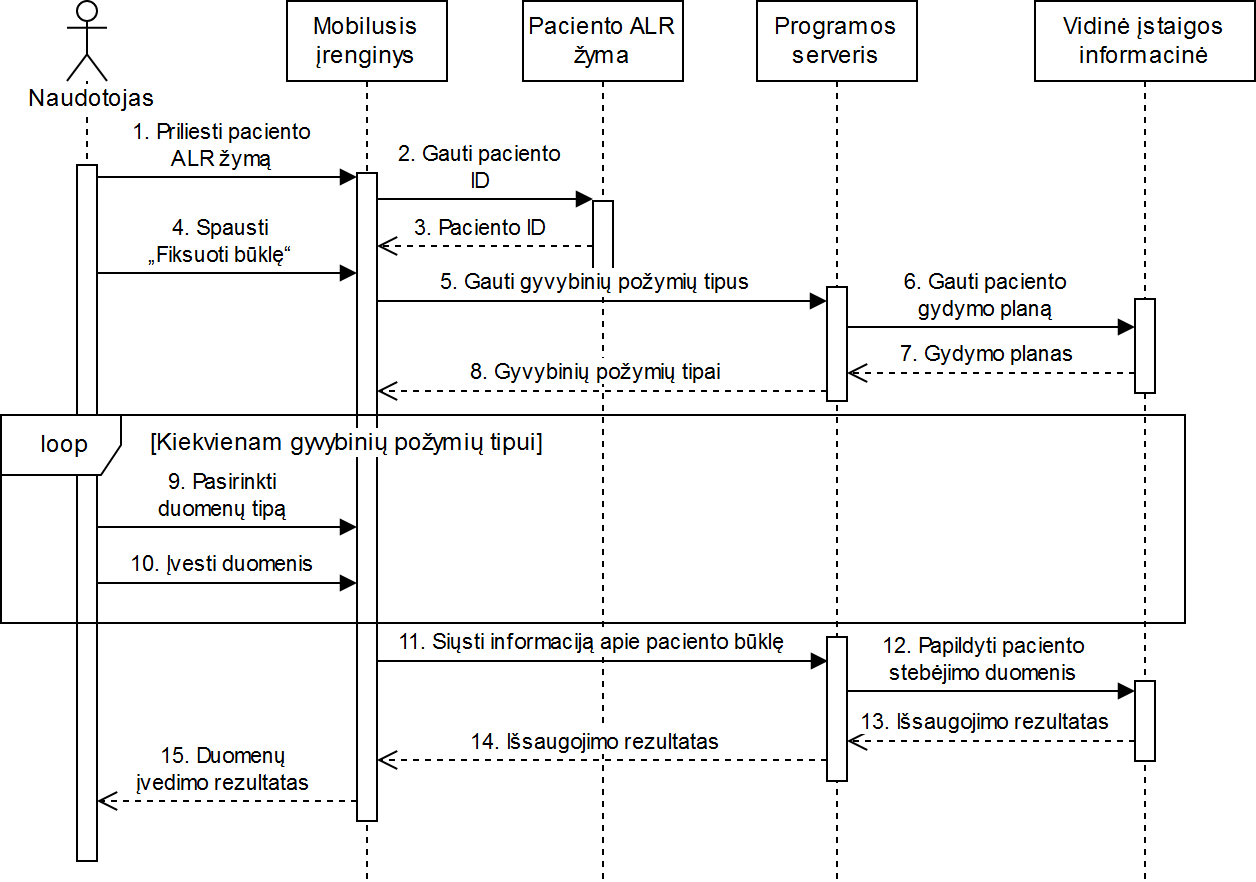
\includegraphics[scale=0.27]{images/buklesFiksavimas}
    \caption{Paciento būklės fiksavimas sekų diagrama} 
\end{figure}

Pateikta paciento būklės fiksavimo diagrama nurodo žingsnius, reikalingus užfiksuoti gautus būklės duomenis, tačiau žingsnių kiekis gali būti mažesnis, todėl toliau aptariamos šios sekų diagramos žingsnių alternatyvos.

\textbf{Paciento gydymo plano informaciją laikyti ALR žymoje}. Ši alternatyva taip pat minima medikamentų išdavimo žingsnių alternatyvose (žiūrėti 4.2.4. poskyrį), todėl argumentai, kodėl ši alternatyva nėra pasirinkta, išlieka tie patys.

\textbf{Atsisakyti gyvybinio požymio tipo pasirinkimo}. Atsisakius šio žingsnio, naudotojui nereiktų patikslinti kokie duomenys yra įvesti, t.y. ar įvesti kūno temperatūros rodikliai, ar kraujo ritmo ir t.t. Naudotojui pakaktų įvesti tinkamo formato duomenis, o sistema pagal duomenų formatą, juos validuotų ir priskirtų jiems gyvybinio požymio tipą. Pasirinkus šią alternatyvą, pirminiam agentui sumažėtų žingsnių kiekis, tačiau padidėtų duomenų formato klaidų tikimybė. Jeigu naudotojas įveda paciento kūno temperatūros duomenis širdies ritmo rodiklio formatu, sistema supranta, kad įvesti širdies ritmo duomenys, o ne kūno temperatūros.

\subsubsection{Informacinis vaizdas}
Informacinio vaizdo pateikimui naudojama esybių ryšių diagrama, kuri nusako esybes ir ryšius tarp jų. Informacinis vaizdas yra pateiktas žemiau (žiūrėti 6 pav.), esybių aprašymas yra pateiktas lentelėje (žiūrėti 5 lentelę).

\begin{figure}[H]
    \centering
    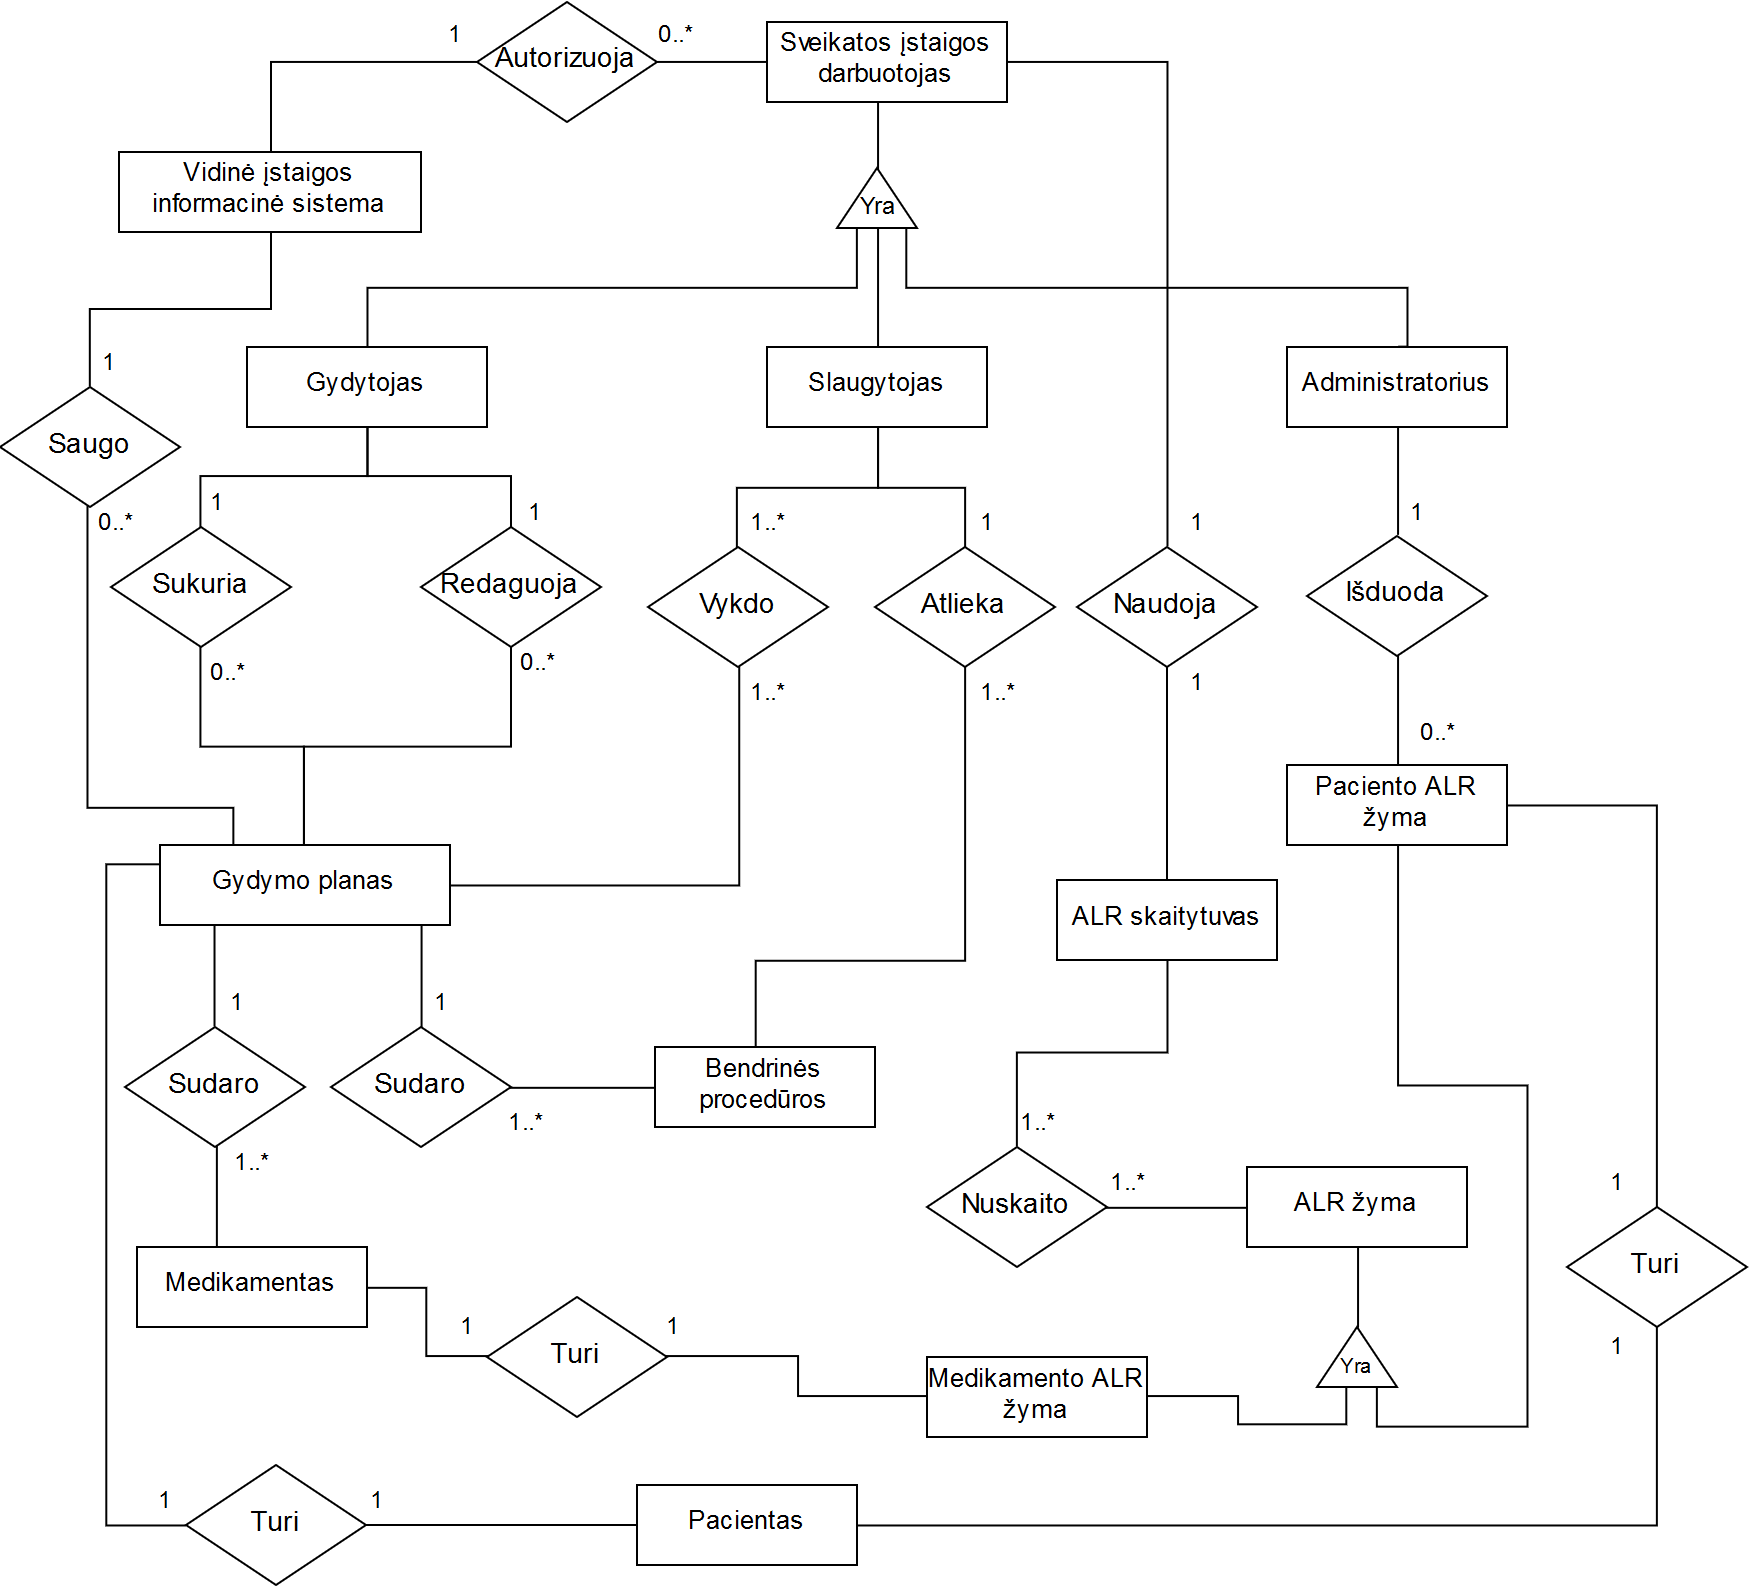
\includegraphics[scale=0.27]{images/erDiagrama}
    \caption{Esybių ryšių diagrama}
\end{figure}

\begin{table}[!ht]
    \centering
    \renewcommand{\arraystretch}{1.2}
    \renewcommand\thetable{7}
    \caption{Esybių aprašymas} 

    \begin{tabular}{|m{3em}|m{12em}|m{22em}|}
    \hline 
    \rowcolor[HTML]{EFEFEF} 
    Nr. & Esybė & Aprašymas \\ \hline

    1  &  Sveikatos įstaigos darbuotojas  & Abstrakti klasė, kuri apibūdina įstaigos darbuotojus      \\ \hline
    2  &  Gydytojas  & Informacija apie sveikatos įstaigos darbuotoją, kuris yra kvalifikuotas paskirti gydymą     \\ \hline
    3  &  Slaugytojas  & Informacija apie sveikatos įstaigos darbuotoją, kuris prižiūri pacientus ir padeda juos gydyti    \\ \hline
    4  &  Administratorius  & Informacija apie sveikatos įstaigos darbuotoją, kuris administruoja ALR žymų išdavimą       \\ \hline
    5  &  Vidinė įstaigos informacinė sistema  & Vidinė įstaigos informacinė sistema, kuri autorizuoja sistemos naudotojus ir saugo duomenis \\ \hline
    6  &  Gydymo planas  & Informacija apie paskirtą gydymą. Gydymo plane nurodomos reikalingos procedūros, reikalingi medikamentai ir tyrimai       \\ \hline
    7  &  Medikamentas  & Informacija apie medikamentą       \\ \hline
    8  &  Bendrinė procedūra  & Informacija apie stacionaraus gydymo bendrinę procedūrą       \\ \hline
    9  &  Pacientas  & Klinikiniai paciento duomenys       \\ \hline
    10  &  ALR žyma  & Abstrakti klasė, kuri apibūdina naudojamas ALR žymas    \\ \hline
    11  &  Paciento ALR žyma  & Informacija apie paciento ALR žymą, joje saugomas paciento identifikacijos numeris    \\ \hline
    12  &  Medikamento ALR žyma  & Informacija apie medikamento ALR žymą, joje saugomas medikamento identifikacijos numeris, galiojimo pabaigos data    \\ \hline
    13  &  ALR skaitytuvas  & Informacija apie stacionariame gydyme naudojamą ALR skaitytuvą \\ \hline

    % 4  &  Administratorius  & Informacija apie sveikatos įstaigos darbuotojas, kuris administruoja ALR žymų išdavimą.       \\ \hline
    % 5  &  Vidinė įstaigos informacinė sistema  & Vidinė įstaigos informacinė sistema, kuri autorizuoja sistemos naudotojus ir saugo duomenis \\ \hline
    % 6  &  Gydymo planas  & Informacija apie paskirtą gydymą. Gydymo plane nurodomos reikalingos procedūros, reikalingi medikamentai ir tyrimai.       \\ \hline
    % 7  &  Medikamentas  & Informacija apie medikamentą.       \\ \hline
    % 8  &  Bendrinė procedūra  & Informacija apie stacionaraus gydymo bendrinę procedūrą.       \\ \hline
    % 9  &  Pacientas  & Klinikiniai paciento duomenys.       \\ \hline
    % 10  &  ALR žyma  & Abstrakti klasė, kuri apibūdina naudojamas ALR žymas.    \\ \hline
    % 11  &  Paciento ALR žyma  & Informacija apie paciento ALR žymą, joje saugomas paciento indentifikacijos numeris.    \\ \hline
    % 12  &  Medikamento ALR žyma  & Informacija apie paciento ALR žymą, joje saugomas paciento indentifikacijos numeris, galiojimo pabaigos data.    \\ \hline
    % 13  &  ALR skaitytuvas  & Informacija apie stacionariame gydyme naudojamą ALR skaitytuvą. \\ \hlin

    \end{tabular}

\end{table}

% \begin{table}[ht!]
%     \centering
%     \renewcommand{\arraystretch}{1.2}
%     \renewcommand\thetable{7}

%     \begin{tabular}{|m{3em}|m{12em}|m{22em}|}
%     \hline 
%     \rowcolor[HTML]{EFEFEF} 
%     Nr. & Esybė & Aprašymas \\ \hline

%     % 1  &  Sveikatos įstaigos darbuotojas  & Abstrakti klasė, kuri apibūdina įstaigos darbuotojus.      \\ \hline
%     % 2  &  Gydytojas  & Informacija apie sveikatos įstaigos darbuotojas, kuris yra kvalifikuotas paskirti gydymą.     \\ \hline
%     % 3  &  Slaugytojas  & Informacija apie sveikatos įstaigos darbuotojas, kuris prižiūri pacientus ir padeda juos gydyti.    \\ \hline
%     4  &  Administratorius  & Informacija apie sveikatos įstaigos darbuotoją, kuris administruoja ALR žymų išdavimą       \\ \hline
%     5  &  Vidinė įstaigos informacinė sistema  & Vidinė įstaigos informacinė sistema, kuri autorizuoja sistemos naudotojus ir saugo duomenis \\ \hline
%     6  &  Gydymo planas  & Informacija apie paskirtą gydymą. Gydymo plane nurodomos reikalingos procedūros, reikalingi medikamentai ir tyrimai       \\ \hline
%     7  &  Medikamentas  & Informacija apie medikamentą       \\ \hline
%     8  &  Bendrinė procedūra  & Informacija apie stacionaraus gydymo bendrinę procedūrą       \\ \hline
%     9  &  Pacientas  & Klinikiniai paciento duomenys       \\ \hline
%     10  &  ALR žyma  & Abstrakti klasė, kuri apibūdina naudojamas ALR žymas    \\ \hline
%     11  &  Paciento ALR žyma  & Informacija apie paciento ALR žymą, joje saugomas paciento identifikacijos numeris    \\ \hline
%     12  &  Medikamento ALR žyma  & Informacija apie medikamento ALR žymą, joje saugomas medikamento identifikacijos numeris, galiojimo pabaigos data    \\ \hline
%     13  &  ALR skaitytuvas  & Informacija apie stacionariame gydyme naudojamą ALR skaitytuvą \\ \hline


%     \end{tabular}

% \end{table}

\subsubsection{Dislokavimo vaizdas}
Dislokavimo vaizdo pateikimui naudojama dislokavimo diagrama, kuri nurodo projektuojamos sistemos elementų išsidėstymą aparatinėje įrangoje. Dislokavimo vaizdas yra pateiktas žemiau (žiūrėti 7 pav.).
\begin{figure}[H]
    \centering
    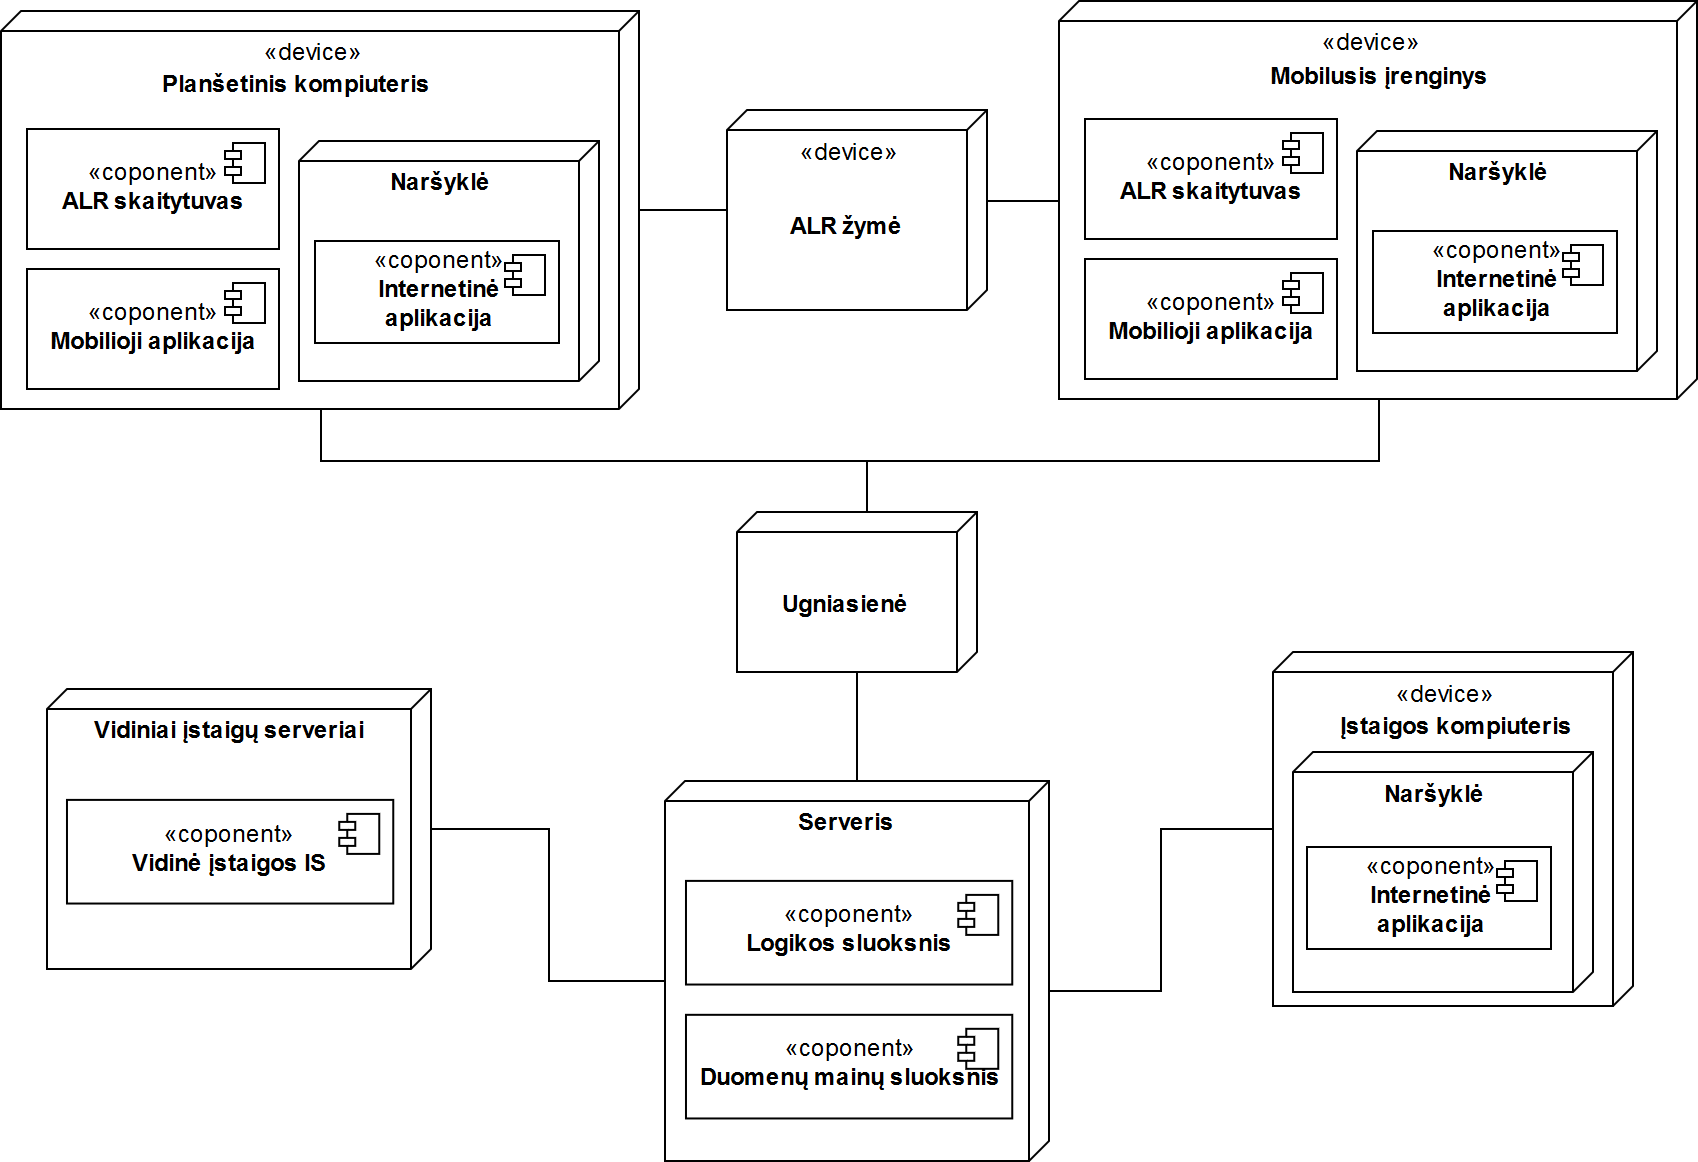
\includegraphics[scale=0.27]{images/deployment}
    \caption{Dislokavimo diagrama}
\end{figure}

\subsubsection{Plečiamumo taškai}
Tam, kad sistema būtų ilgaamžė ir įgyvendintų naujai keliamus reikalavimus, labai svarbus yra sistemos plečiamumas \cite{Bass2013}. Pagrindiniai projektuojamos sistemos plečiamumo taškai: 
\begin{itemize}
    \item Integravimasis su naujomis informacinėmis sistemomis;
    \item Sensorių, kurie matuoja pacientų gyvybines funkcijas, pridėjimas;
    \item Pridėti ALR darbo režimą - vartotojas vartotojui.
\end{itemize}

\textbf{Integravimasis su naujomis informacinėmis sistemomis}. Kadangi projektuojama sistema yra priklausoma nuo išorinių sistemų teikiamų duomenų apie pacientą ir įstaigos darbuotojus, pagrindinis plėtimo taškas - integravimasis su šiomis sistemomis. Projektuojamoje sistemoje yra apibrėžtas duomenų mainų sluoksnis arba integracinis sluoksnis. Atliekant integraciją, duomenų mainų sluoksnis turėtų teikti projektuojamai sistemai vienareikšmiškus duomenis, tarp skirtingų įstaigų, duomenų struktūra neturi keistis. Išorinių sistemų teikiamų paciento duomenų struktūra turėtų atitikti HL7 standartą, tačiau jeigu šio standarto duomenys neatitinka, reikalingi duomenų sluoksnio pakeitimai. Kiekvieno integravimo metu, moduliams, kurie atsakingi už įstaigos darbuotojų duomenų adaptavimą, bus reikalingi pakeitimai, nes šiems duomenis nėra bendro standarto.

\textbf{ALR sensorių, kurie matuoja pacientų gyvybines funkcijas, pridėjimas}. Nagrinėtoje literatūroje analizuojamas gyvybines funkcijas matuojančių ALR sensorių panaudojimas \cite{Strommer2006}. Kadangi siūlomoje sistemoje visus paciento gyvybinius požymius įveda slaugos darbuotojas, vienas iš sistemos plėtimo taškų - ALR sensorių, kurie matuoja pacientų gyvybines funkcijas, įdiegimas. Šių sensorių diegimas turėtų įtakos mobiliajai aplikacijai. Diegiant sensorius, reikėtų atlikti mobiliosios aplikacijos pakeitimus, t.y. gavus duomenis iš sensoriaus, jie automatiškai užpildytų gyvybinių požymių formos laukus. Šių sensorių pridėjimas neturi daryti įtakos vidiniai sistemos daliai.

\textbf{Pridėti ALR darbo režimą - vartotojas vartotojui}. Taip pat vienas iš plėtimo taškų - vietoj ALR žymos, naudoti ALR įrenginius, t.y. įgalinti vartotojas vartotojui darbo režimą. Šis darbo režimas leistų laikyti konfidencialius paciento duomenis ALR įrenginyje. Norint įdiegti šį darbo režimą, siūlomoje sistemoje reikalingi mobiliosios aplikacijos pakeitimai.



\subsection{Projektuojamos sistemos prototipas}
Šiame poskyryje yra aprašomas projektuojamos sistemos prototipas. Prototipo tikslas - išsiaiškinti ar pagrindinius sistemos scenarijus įmanoma įgyvendinti. Šiame poskyryje pirmiausiai aprašomi prototipo uždaviniai, po to aprašoma realizacija ir prototipo testavimas.

\subsubsection{Uždaviniai}
Prototipo tikslui pasiekti išsikelti šie uždaviniai:

\begin{itemize}
    \item Nuskaityti paciento ALR žymą;
    \item Nuskaityti medikamento ALR žymą;
    \item Gauti paciento gydymo planą;
    \item Užfiksuoti paciento būklę;
    \item Verifikuoti medikamento išdavimą.
\end{itemize}

\subsubsection{Realizacija}
Prototipo įgyvendinimui buvo pasirinkti „React Native“ ir „Express.js“ karkasai. „React Native“ skirtas kurti mobiliąsias aplikacijas. Šis karkasas pasirinktas dėl to, kad parašius aplikacijos kodą „Javascript“ programavimo kalba, karkasas pasirūpina, kad aplikacija veiktų tiek „iOS“, tiek „Android“ operacinėse aplinkose, todėl nereikia kurti dviejų atskirų aplikacijų, kurios būtų pritaikytos šioms dviems operacinėms sistemoms. „Express.js“ skirtas kurti vidinę sistemos dalį. Šis karkasas buvo pasirinktas dėl to, kad programinis kodas yra rašomas su „Javascript“ programavimo kalba, todėl sistemos tiek išorinė, tiek vidinė dalis yra rašoma ta pačia programavimo kalba. Šis karkasas taip pat leidžia greitai kurti vidinę sistemos dalį, o kadangi kuriamas sistemos prototipas, „Express.js“ tinka išsikeltiems uždaviniams atlikti.


Pirmiausiai buvo kuriama vidinė sistemos dalis. Kadangi siūloma, jog duomenų saugojimas būtų vykdomas sveikatos įstaigų vidinių sistemų pagalba, duomenų saugojimui nebuvo kuriama duomenų bazė, o duomenys saugomi failinėje sistemoje. Vidinėje sistemos dalyje buvo sukurti 4 galutiniai taškai (angl. \textit{endpoint}), kurie priima mobiliosios aplikacijos užklausas ir grąžina atsakymą. Šie galutiniai taškai atlieka šiuos funkcionalumus: 
\begin{itemize}
    \item Patikrina ar išduodamas tinkamas medikamentas;
    \item Grąžina pacientui aktualius gyvybinių požymių tipus;
    \item Priima ir išsaugo informaciją apie paciento būklę;
    \item Grąžina visą informaciją, kuri susijusi su pacientu. Šį funkcionalumą atliekantis galutinis taškas yra naudojamas testuojant sistemos veikimą.
\end{itemize}
Sukūrus vidinę sistemos dalį, buvo kuriama mobilioji aplikacija. Tam, kad aplikacija galėtų pasiekti nuskaitytus ALR žymos duomenis, buvo pasirinkta naudoti „react-native-nfc-manager“ biblioteka, kuri palengvina darbą su ALR technologija. Nuskaičius ALR žymą ir gavus joje esančius duomenis, aplikacija iškoduoja gautus duomenis. Turint paciento ID, pagal naudotojo pasirinkimą, aplikacija arba laukė kol nuskaitys medikamento ALR žymą, arba gavus pacientui aktualius gyvybinių požymių tipus, laukė kol vartotojas suves informaciją apie paciento būklę (žiūrėti8 pav., 9 pav., 11pav., 12pav. ). Turint visą reikiamą informaciją, aplikacija kreipėsi į vidinę sistemos dalį (žiūrėti 11 pav., 13 pav.).



\subsubsection{Testavimas}

Sukūrus prototipą, testavimas buvo atliekamas 3 etapais:
\begin{enumerate}
    \item Mobiliosios aplikacijos funkcionalumo testavimas;
    \item Vidinės sistemos dalies funkcionalumo testavimas;
    \item Pagrindinių sistemos scenarijų testavimas;
\end{enumerate}

Sistemos prototipo testavimo metu buvo naudojami šie įrenginiai:
\begin{itemize}
    \item Mobilusis įrenginys Nokia 6.1 su Android 9 operacine sistema;
    \item Mobilusis įrenginys Samsung Galaxy S6 su Android 7 operacine sistema;
    \item Mobilusis įrenginys Iphone 8 su iOS 11 operacine sistema;
    \item 4 NXP MIFARE Ultralight C ALR žymos, kurios paremtos ISO 14443-3A standartu.
\end{itemize}

Testuojant mobiliąją aplikaciją, pirmiausiai buvo testuojamas ALR žymų nuskaitomumas. Visi 3 mobilieji įrenginiai sugebėjo nuskaityti duomenis esančius ALR žymoje. Ištestavus ALR nuskaitomumą, pradėta testuoti tinkamų vaizdų parodymus aplikacijoje ir komunikavimas su vidine sistemos dalimi. Nors mobiliajame įrenginyje, kuris turi iOS operacinę sistemą, mobiliosios aplikacijos vaizdai nežymiai skyrėsi nuo Android įrenginių, tačiau tai neturėjo įtakos mobiliosios aplikacijos funkcionalumui.

Testuojant vidinės sistemos dalies funkcionalumą, buvo naudojamas „Postman“ įrankis. Kadangi vidinės sistemos dalies pagrindinis funkcionalumas - priimti, verifikuoti ir išsaugoti duomenis, buvo pakartotinai siuntinėjamos įvairios užklausos su tinkamais ir netinkamais duomenimis.

Pagrindinių sistemos scenarijų testavimo metu su skirtingais įrenginiais buvo atliekami 4 skyriuje aprašyti scenarijai. Pirmiausiai su „NFC tool“ įrankiu buvo paruošiamos 2 pacientų ALR žymos ir 2 medikamentų ALR žymos. Su visais 3 mobiliais įrenginiais buvo tikrinamas medikamentų verifikavimas ir pacientų būklės fiksavimas. Atlikus testavimus paaiškėjo, jog pagrindinius sistemos scenarijus įmanoma įgyvendinti, todėl išsikeltas prototipo tikslas buvo pasiektas.